\input ../SlidePreamble
\input ../preamble

\begin{document}

{\Huge

  \centerline{\bf TTIC 31230, Fundamentals of Deep Learning}
  \bigskip
  \centerline{David McAllester, Winter 2020}

\vfill
  \centerline{\bf The free Lunch Theorem}
  \vfill
  \centerline{\bf and The Intelligence Explosion}
  \vfill
  \vfill

\slide{The Free Lunch: Chomsky vs. Kolmogorov}

\includegraphics[width=1.0 in]{../images/Chomsky} \begin{minipage}[b]{8in} Noam Chomsky: 
  By the no free lunch theorem {\bf natural language grammar is unlearnable without an innate linguistic capacity}. In any domain a strong prior (a learning bias)
  is required. \end{minipage}

\vfill
\includegraphics[height=1.0 in]{../images/Levin}
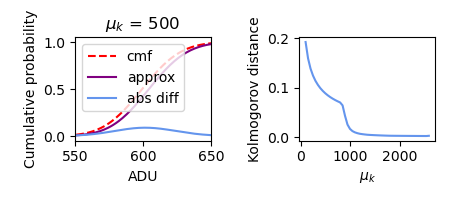
\includegraphics[height=1.0 in]{../images/Kolmogorov}
\includegraphics[height=1.0 in]{../images/Hinton}
\includegraphics[height=1.0 in]{../images/Schmidhuber}

\begin{minipage}[b]{7in}
  Leonid Levin, Andrey Kolmogorov, Geoff Hinton and J\"{u}rgen Schmidhuber: {\bf Universal learning algorithms exist.
  No domain-specific innate knowledge is required.}
\end{minipage}

\slide{The Free Lunch Theorem}

Consider any fixed language for naming functions. For example C++. (or English?)

\vfill
Let $|f|$ be the number of bits it takes to name function $f$ in that langauge.

\vfill
For $z \sim \pop$, let ${\cal L}(f,z) \in [0,L_{\mathrm{max}}]$ be a bounded loss function.

\vfill
{\bf Free Lunch Theorem:} With probability at least $1-\delta$ over the draw of training data $z_1,\;\ldots,\;z_N$ from $\pop$,
the following holds {\em simultaneously} for all nameable functions $f$
$${\cal L}(f) \leq\frac{10}{9}\parens{\widehat{\cal L}(f) + \frac{5L_{\mathrm{max}}}{N}\parens{(\ln 2)|f| + \ln\frac{1}{\delta}}}$$

\slide{The Intelligence Explosion}

Another kind of free lunch:

\vfill
\begin{quotation}
Let an ultraintelligent machine be defined as a machine that can far surpass all the intellectual activities of any person however clever. Since the design of machines is one of these intellectual activities, an ultraintelligent machine could design even better machines; there would then unquestionably be an ‘intelligence explosion,’ and the intelligence of humanity would be left far behind. Thus the first ultraintelligent machine is the last invention that humanity need ever make, provided that the machine is docile enough to tell us how to keep it under control.
\end{quotation}

\vfill
\rightline{I.J. Good, 1969}
\slide{The Baldwin Effect: Learning Facilitates Adaptation}

\includegraphics[width = 1.2in]{../images/hinton}

In a 1987 paper entitled ``How Learning Can Guide Evolution'', Goeffrey Hinton and Steve Nowlan brought attention to a paper by Baldwin (1896).

\vfill
The basic idea is that by facilitating adaptation of the individual, learning facilitates evolution of the species.

\vfill
For example, longer arms are easier to evolve if arm control is learned --- arm control is then independent of arm length.  Arm control and arm structure become more modular.

\slide{The Meta-Baldwin Effect: Learning Facilitates Learning}

The Baldwin effect should apply to brain modules as well, such as vision or the motor cortex.

\vfill
By facilitating adaptation of the individual during its lifetime, learning facilitates both the evolution of the use of a module as well
as evolution of the module itself.

\slide{Levin's Universal Problem Solver}

\includegraphics[height=2.0 in]{../images/Levin}
Leonid Levin observed that one can construct a universal solver.  The solver takes as input a solution tester
and returns as output a solution whenever a solution exists.

  \vfill
Levin's solver is universal in the sense that it is not more than a constant factor slower than any other solver mapping testers to solutions.

\vfill
It follows that for any problem in NP, the universal solver provides a P-time algorithm whenever any such algorithm exists.


\slide{Levin's Universal Solver}
  
\vfill
We time share all programs giving time slice $2^{-|h|}$ to program $h$ where $|h|$
is the length in bits of $h$.

\vfill
The run time of the universal solver is at most
$$O(2^{-|h|}(h(n) + T(n)))$$
where $h(n)$ is the time required to run program $h$ on a problem of size $n$ and $T(n)$ is the time required to check the solution.

\vfill
Here $2^{-|h|}$ is independent of $n$ and is technically a constant.

\slide{Learning the Universal Solver}
\vfill
\includegraphics[width= 1in]{../images/schmidhuber}
Schmidhuber proposes a learning algorithm for learning an optimal universal solver.
The Optimally Ordered Problem Solver (OOPS), Schmidhuber, 2002.


\slide{Levin and Schmidhuber}
  
\vfill
We time share all programs giving time slice $2^{-|h|}$ to program $h$ where $|h|$
is the length in bits of $h$.

\vfill
Both Levin's universal solver and Schmidhuber's optimal problem solver involve exponentially large constants.

\vfill
There seems to be little insight here beyond that of I.J. Good's original formulation of the intelligence explosion.

\slide{END}

}
\end{document}
